\documentclass[amsmath,amssymb,notitlepage,11pt]{revtex4-1}
%\documentclass[12pt]{article}
\usepackage{graphicx}
\usepackage{bm}% bold math
\usepackage{multirow}
\usepackage{booktabs}
\usepackage{verbatim}
\usepackage{hyperref}
\usepackage{enumitem}
\hypersetup{pdftex,colorlinks=true,allcolors=blue}
\usepackage{hypcap}
\usepackage[small,compact]{titlesec}
\setlist[enumerate]{itemsep=0mm}

\begin{document}
\title{HPS Chicane Operations Manual v1.4}
\author{N. Baltzell}
\affiliation{Jefferson Lab}
\date{\today}
\begin{abstract}
    Controls of the HPS chicane are updated for 2016 to simplify operations during shift.  This includes a simplified user interface, automatic retrieval of beam energy, automatic calculations of magnet current setpoints based on~\cite{chicaneSettings}, and EPICS sequencers to energize and disable all HPS chicane magnets with minimal user interaction.  This manual explains the operations of the new interface. 
\end{abstract}
%\hspace*{11.5cm}\texttt{HPS-NOTE 2015-XXX}

%\affiliation{Jefferson Lab}
\maketitle
\tableofcontents
\newpage

\section{Overview}
The new chicane screen is accessiable from the main HPS-EPICS screen, under {\em Magnets}$ \to$ {\em Chicane}, and shown in Figure~\ref{fig:guiChicaneOff}.  It contains a few buttons and many readbacks describe in the following subsections.  Displayed numbers are in units Amps, Gauss, or MeV. 
\begin{figure}[htbp]
    \centering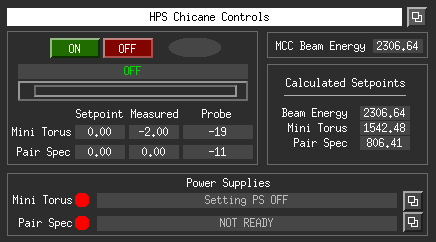
\includegraphics[width=12cm]{pics/guiOFF}
    
    \centering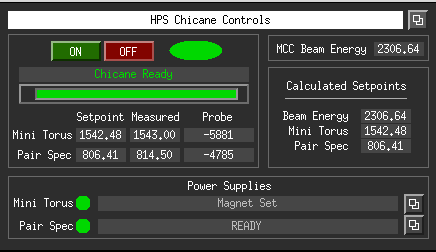
\includegraphics[width=12cm]{pics/guiON}
    \caption{The new chicane screen with both magnets' power supplies off (top), and with chicane energized and ready for 2.306 GeV beam (bottom).\label{fig:guiChicaneOff}}
\end{figure}
\subsection{Buttons}
This GUI contains five buttons:
\begin{enumerate}
    \item The basic {\em ON} and {\em OFF} buttons, which is all the general shift worker should need for controls.
    \item One expert button in the top right corner for customization of chicane setpoints.
    \item Two expert buttons in the bottom right corner that are just links to the magnets' power supplies' old expert screens.
\end{enumerate}
\subsection{Readbacks}
This GUI also contains various readback values:
\begin{enumerate}
    \item In the top left is a global status message and a corresponding progress bar.
    \item Below that are setpoints and measured currents from the magnets' power supplies, and our Hall probes' readback values.
    \item In the top right is the beam energy currently being reported from MCC, and the beam energy and magnet current calculations currently being used by this software to set HPS's magnets.
    \item The bottom portion of the screen is status readbacks from the power supplies.  These are a summary from the magnets' two expert screens.
\end{enumerate}

\section{Shifters Operations}
This is all that shift workers need to operate the chicane:  ``On'' and ``Off''.  {\bf\em At the beginning of the sequences, it is advised to confirm the main message box and setpoint and measured current have reasonable behavior.  Particularly, that the measured magnet currents begin to ramp up/down within a minute after pressing the ON/OFF buttons.}
\subsection{On}
To turn the chicane on, press the green {\em ON} button.  That will begin a sequence to energize the magnets and eventually bring them to the desired ``calculated'' setpoints shown in the top right of the GUI.  After that is accomplished the main message bar will display ``Chicane Ready'' and you are then ready for beam.  This will take a total of about {\bf 40 minutes} between the time {\em ON} is pressed and ``Chicane Ready'' is achieved.  The details of the {\em ON} sequence are described in the next section.
\subsection{Off}
To turn the chicane off, press the red {\em OFF} button.  That will begin a sequence to ramp the magents down to zero current and then switch the power supplies off.  Then the main message box should dislay ``OFF''.  This will take a total of about {\bf 10 minutes}.  The details of the ``OFF'' sequence are described in the next section.
\newpage
\section{Sequence Details}
\subsection{On}
The ``On'' button will intiate the procedure to go from chicane off to beam ready.
\begin{enumerate}
    \item turn both power supplies on
    \begin{itemize}
    \item the main message box will display which supply it is turning on
    \end{itemize}
    \item ramp both power supplies up to their max current
    \begin{itemize}
    \item the main message box will display ``Ramping up to Max''
    \item the current setpoints will get updated to 2700A/3500A for the PairSpec/Frascatis
    \item the progress meter will display progress towards setpoint currents
    \item the measured currents will gradually increase
    \end{itemize}
    \item saturate at max current for N minutes
    \begin{itemize}
    \item the main message box will display ``Saturating for \# seconds''
    \item the progress meter will display fraction of soak time remaining  
    \item the setpoint and measured currents should remain stable 
    \end{itemize}
    \item ramp both power supplies down to their calculated setpoints
    \begin{itemize}
    \item the main message will display ``Ramping Down to Setpoint''
    \item the current setpoints will get updated to the calculated values
    \item the measured currents will gradually decrease towards the new setpoints
    \end{itemize}
    \item display ``Ready'' in the main message box once measured currents match the setpoints
\end{enumerate}
{\em Currently the countdown for saturation time begins when the PairSpec magnet reaches max current.  This was done to conserve time, because Frascati magnets ramp more slowly than the PairSpec but require much less soak time (7 minutes) compared to the PairSpec (30 minutes).}
\subsection{Off}
The ``Off'' button will initiate the procedure to turn the chicane off.  This would normally be done any time the magnets need to be set to zero.
\begin{enumerate}
    \item ramp both power supplies down to zero current
    \begin{itemize}
    \item the main message box will display ``Ramping to Zero''
    \item the progress meter will display progress towards zero current
    \item the setpoints will get updated to 8A/0A for PairSpec/Frascatis
    \item the measured currents will gradually decrease
    \end{itemize}
    \item turn both power supplies off
    \begin{itemize}
    \item the main message box will display which supply it is turning off
    \end{itemize}
    \item display ``OFF'' in the main message box
\end{enumerate}

\section{Expert Operations}
\subsection{Expert Screen}
This expert screen, shown in Figure~\ref{fig:expert}, is accessible from the top right button in the main chicane screen (Figure~\ref{fig:guiChicaneOff}).  It was created after seeing what primary expert operations were done during the 2016 run:  manually tuning the magnets' current settings.  This can be done in the left column under ``Live''.  What should additionally be done in the future, after calibrating the settings manually, is to input those same settings in the ``Saved'' column such that they are restored the next time the chicane is turned on. 
\begin{figure}[htbp]\centering
    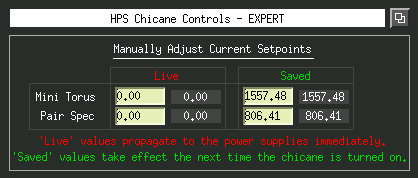
\includegraphics[height=5cm]{pics/expertA}
    \caption{The Expert screen.  Here both power supplies are off and the ``Live'' setpoints are zero.  The ``Saved'' setpoints will take effect automatically the next time the chicane is turned on.\label{fig:expert}}
\end{figure}

\subsection{Super Expert Screen}
The ``super expert'' screen (Figure~\ref{fig:superexpert}) was originally written in anticipation of what would be needed before people actually started using this new system.  It is accessible from a button in the top right of the ``Expert'' screen and has so far not been used during the 2016 run expect for setting the initial chicane currents based on MCC beam energy.
\begin{enumerate}
\item The topmost section is of most importance, calculating the magnet currents from the MCC beam energy.  This uses the relationship between beam energy and magnet currents given in~\cite{chicaneSettings}.
\item
    The second section allows to choose your own beam energy, and then calculate the magnet currents based on beam energy given in~\cite{chicaneSettings}.
\item
The third sections allows to manually scan the magnet currents by adjusting only the beam energy, in accordance with the equations given in~\cite{chicaneSettings}.  This could be useful for a manual scan of chicane settings.
\item
The fourth section just allows to manually input setopints to the power supplies.  This is identical to manually inputting the currents in the expert screens for the individual power supplies.
\item
The last section is some parameters on the sequencer: time to hold for saturation and tolerance to for the sequencer to think measured currents are acceptable.
\end{enumerate}
\begin{figure}[htbp]\centering
    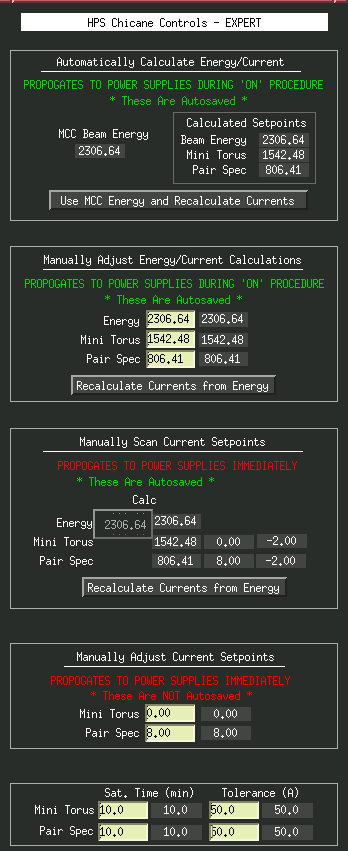
\includegraphics[height=22cm]{pics/expert}
    \caption{The ``Super Expert'' screen.\label{fig:superexpert}}
\end{figure}


\bibliography{ChicaneManual}
\end{document}

